\documentclass{article}

\usepackage{graphicx}
\usepackage[utf8]{inputenc}
\usepackage[T1]{fontenc}
\usepackage[french]{babel}
\usepackage{hyperref}
\usepackage{amsmath,amsfonts,amssymb}
%\usepackage{Tkz-Tab}
\usepackage{wrapfig}
\usepackage{verbatim}
\usepackage{array}

\begin{document}

\title{Gestion de flux dans le réseau
	\smallbreak
	TD n\degre6
	\smallbreak
	Modélisation mathématique
	\smallbreak
	Q4}
\author{Sibylle Roux \and Juliette Arazo \and Nicolas Le Gallo \and Tanguy Thomas}

\maketitle

\newpage

\tableofcontents

\newpage

\section{Etude de la file M/M/1}


\subsection{Conception d'une représentation informatique}
\paragraph{}
Pour stocké les valeurs simulés on utilisera un tableau de la forme : 
\begin{center}
\begin{tabular}{lll}
\hline
\hline
instant $t$ & $q(t)$ & incrément \\
\hline
\hline
\end{tabular}
\end{center}
\paragraph{}
Cette représentation est idéale : elle réunit toutes les informations utiles du fonctionnement des serveurs : 
\begin{itemize}
	\item l'instant où se passe l'evenement
	\item le type d'evenement (entrée ou sortie d'un client dans le système)
	\item le nombres de clients présent dans le système
\end{itemize}
Cette dernière valeur nous sera utile pour avoir la taille de la fille d'attente : 
\begin{align}
	taille\_file=max(q(t)-1,0)
\end{align}

\subsection{Conception et développement d'un algorithme de simulation en scilab}
Nous avons à notre disposition une fonction SciLab $insere(q, ta, ts)$ avec :
\begin{itemize}
	\item \textbf{q} : Matrice de notre représentation informatique de la file
	\item \textbf{ta} : Temps actuel
	\item \textbf{ts} : Temps de service
\end{itemize}
\begin{verbatim}
function newq = insere(q, ta, ts)
    if q($, 1) < ta then 
        q($+1,:) = [ta, 1, 1];
    else
        ind = sum(q(:, 1) < ta);
        q(ind+2:$+1, :) = q(ind+1:$, :);
        q(ind+1,:) = [ta, q(ind,2), 1];
        q(ind+1:$,2) = q(ind+1:$,2) + 1;
    end
    s = q($, 1) + ts 
    q($+1, :) = [s, q($, 2) - 1, -1];
    newq = q
endfunction
\end{verbatim}
\paragraph{}
Nous avons aussi la fonction $randExp(n,lambda)$ qui genere un vecteur de taille $n$ de valeurs aléatoires suivant la loi exponentielle de paramètre $\lambda=lambda$
\begin{verbatim}
function t = randExp(n, lambda)
    t = -log(1 - rand(n,1)) / lambda
endfunction
\end{verbatim}

\paragraph{}
C'est à l'aide de ces deux fonctions citées plus haut que l'on peut définir la fonction : $queue(Tmax, lambda, mu)$ où :
\begin{itemize}
	\item \textbf{Tmax} : Instant maximal de la représentation de la file
	\item \textbf{lambda} : $\lambda$ correspondant aux temps inter-arrivées
	\item \textbf{mu} :  $\lambda$ correspondant aux temps de service
\end{itemize}
\begin{verbatim}
function a=queue(Tmax, lambda, mu)
    Q = [0, 0, 0];
    t = 0; // temps courant
    while (t < Tmax)
        t_ia=randExp(1,lambda);
        t=t+t_ia;
        ts=randExp(1,mu);
        Q=insere(Q,t,ts);
    end
    a = Q (Q(:,1)<Tmax,:)
endfunction
\end{verbatim}

\subsection{Simulation de trajectoires}

\subsubsection{Simulation de l'évolution d'un file d'attente}
\paragraph{}
Pour simuler les différentes trajectoires, on va utiliser une fonction Scilab $traj(n,lambda,mu)$ où :
\begin{itemize}
	\item \textbf{n} : correspondant à l'instant maximal de la représentation de la file
	\item \textbf{lambda} : $\lambda$ correspondant aux temps inter-arrivées
	\item \textbf{mu} :  $\lambda$ correspondant aux temps de service
\end{itemize}
\begin{verbatim}
function traj(n,lambda,mu)
    for i=1:50 // 50 trajectoires
        Q = queue(n, lambda, mu); // lambda est 5 fois plus grand que mu
        plot2d2(Q(:,1), max(Q(:,2) - 1, 0), style=2) // trace la courbe
    end
endfunction
\end{verbatim}

\subsubsection{Distribution statistiques de la taille de la file d'attente}
\paragraph{}
Pour avoir la distribution statistique de des trajectoires, on va utiliser une fonction Scilab $distrib(n,lambda,mu)$ où :
\begin{itemize}
	\item \textbf{n} : correspondant à l'instant maximal de la représentation de la file
	\item \textbf{lambda} : $\lambda$ correspondant aux temps inter-arrivées
	\item \textbf{mu} :  $\lambda$ correspondant aux temps de service
\end{itemize}
\begin{verbatim}
function Qi=distrib(n,lambda,mu)
    Qi = zeros(500, 1);
    for i=1:500
        Q = queue(n, lambda, mu);
        Qi(i) = Q($, 2);
    end
    distr = tabul(Qi,'i')
    bar(distr(:,1),distr(:,2)/500)
    legend("Distribution de Q"+string(n))
endfunction
\end{verbatim}
\paragraph{}
Lorsque l'amplitude sera très grande, on optera plutôt pour une autre version de cette fonction $distribv2(n,lambda,mu)$: 
\begin{verbatim}
function Qi=distribv2(n,lambda,mu)
    Qi = zeros(500, 1);
    for i=1:500
        Q = queue(n, lambda, mu);
        Qi(i) = Q($, 2);
    end
    histplot(20,Qi)
    legend("Distribution de Q"+string(n))
endfunction
\end{verbatim}

\subsubsection{Temps de service supérieur en moyenne aux temps inter-arrivées}
\paragraph{Paramètre : $n=60$ ; $lambda=0.5$ ; $mu=0.2$}
\begin{center}
	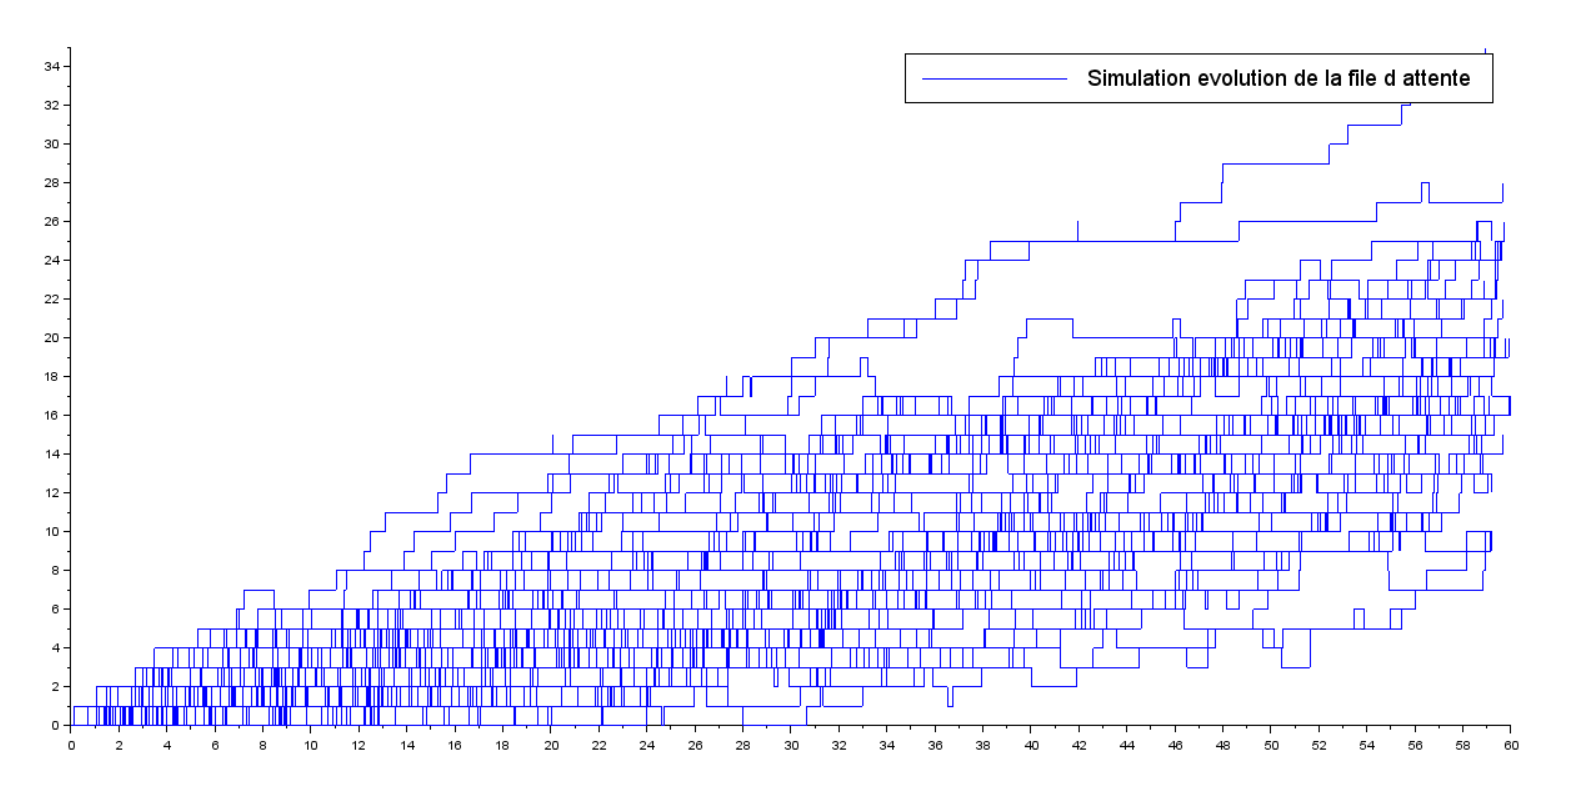
\includegraphics[width=425px]{img/inf.PNG}
\end{center}
\paragraph{} On remarque bien que la file d'attente ne semble pas se stabiliser, mais augmente de manière continue.
\begin{center}
	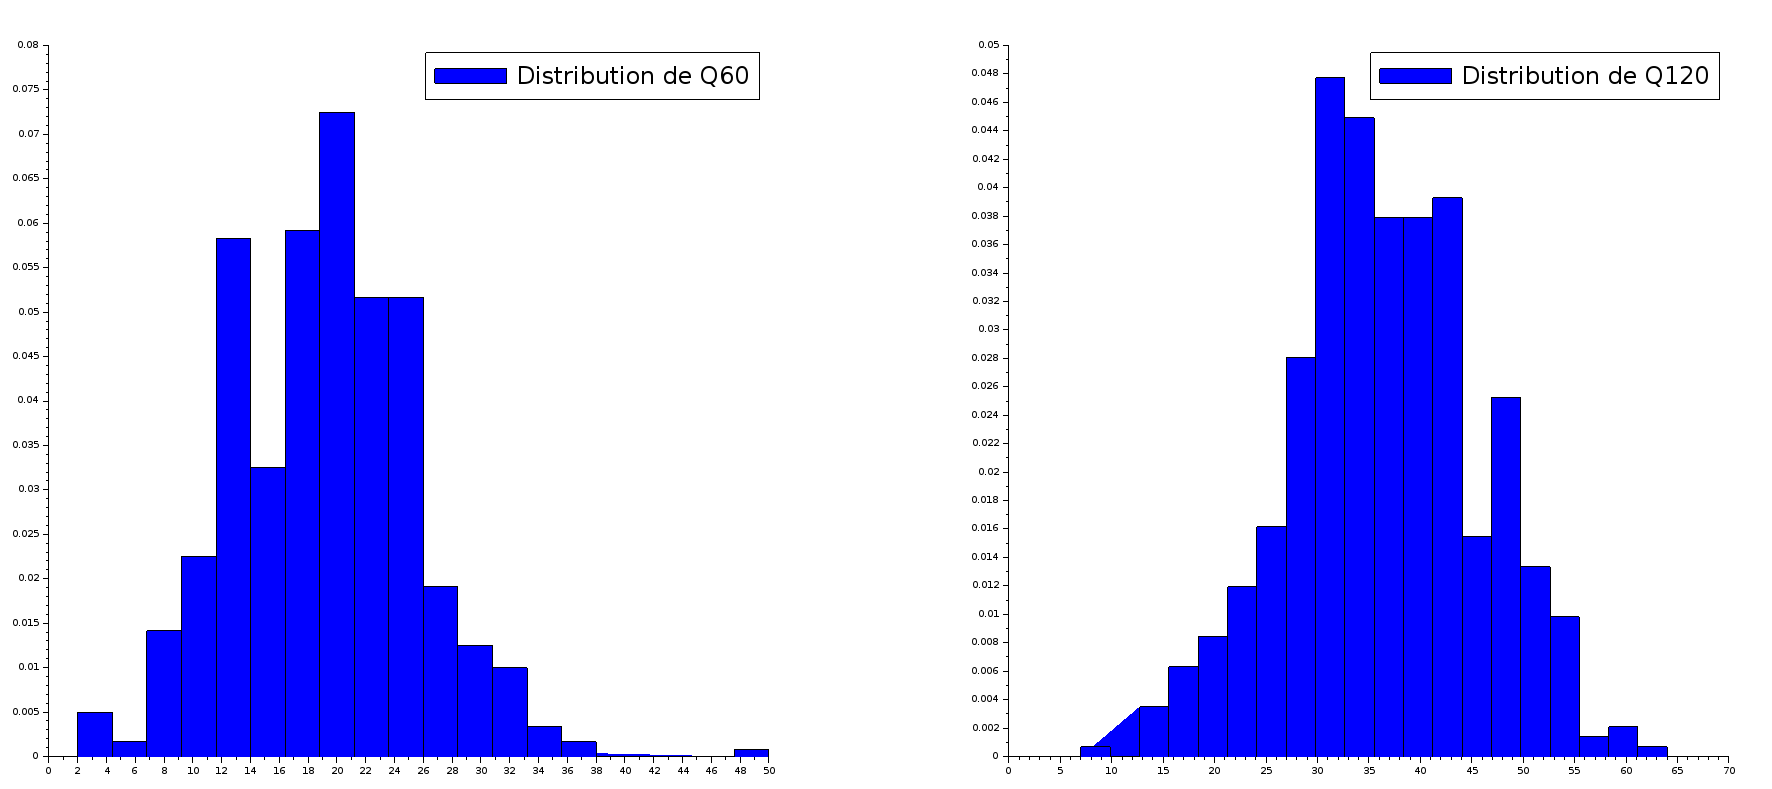
\includegraphics[width=425px]{img/sup/dist.png}
\end{center}

\begin{center}
	\begin{tabular}{c|cc}
		\hline \hline
		& Q60 & Q120 \\
		\hline
		mean() & 18.54 & 36.806 \\
		variance() & 40.212826 & 81.158681 \\
		\hline \hline
	\end{tabular}
\end{center}
\paragraph{}
Quand on étudie la distribution de la file d'attente pour 60 et 120 secondes, on voit bien que les 2 moyennes et variances sont très différents, en effet l'évolution de la file d'attente ne se stabilise pas mais semble augmenter continuellement : $ mean(Q60)<mean(Q120)$.

\subsubsection{Temps de service inférieur en moyenne aux temps inter-arrivées}
\paragraph{Paramètre : $n=60$ ; $lambda=0.2$ ; $mu=0.5$}
\begin{center}
	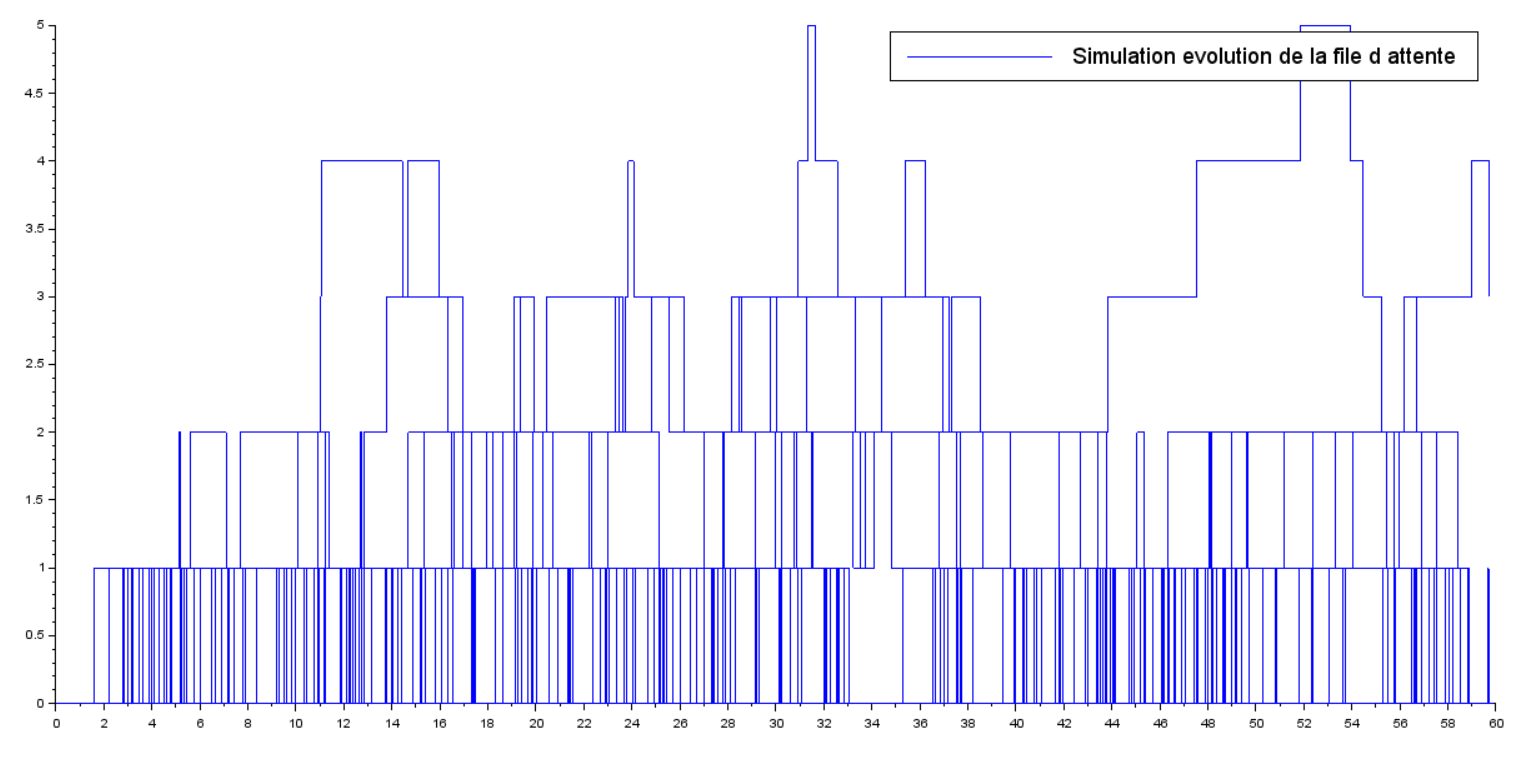
\includegraphics[width=425px]{img/sup.PNG}
\end{center}
\begin{center}
	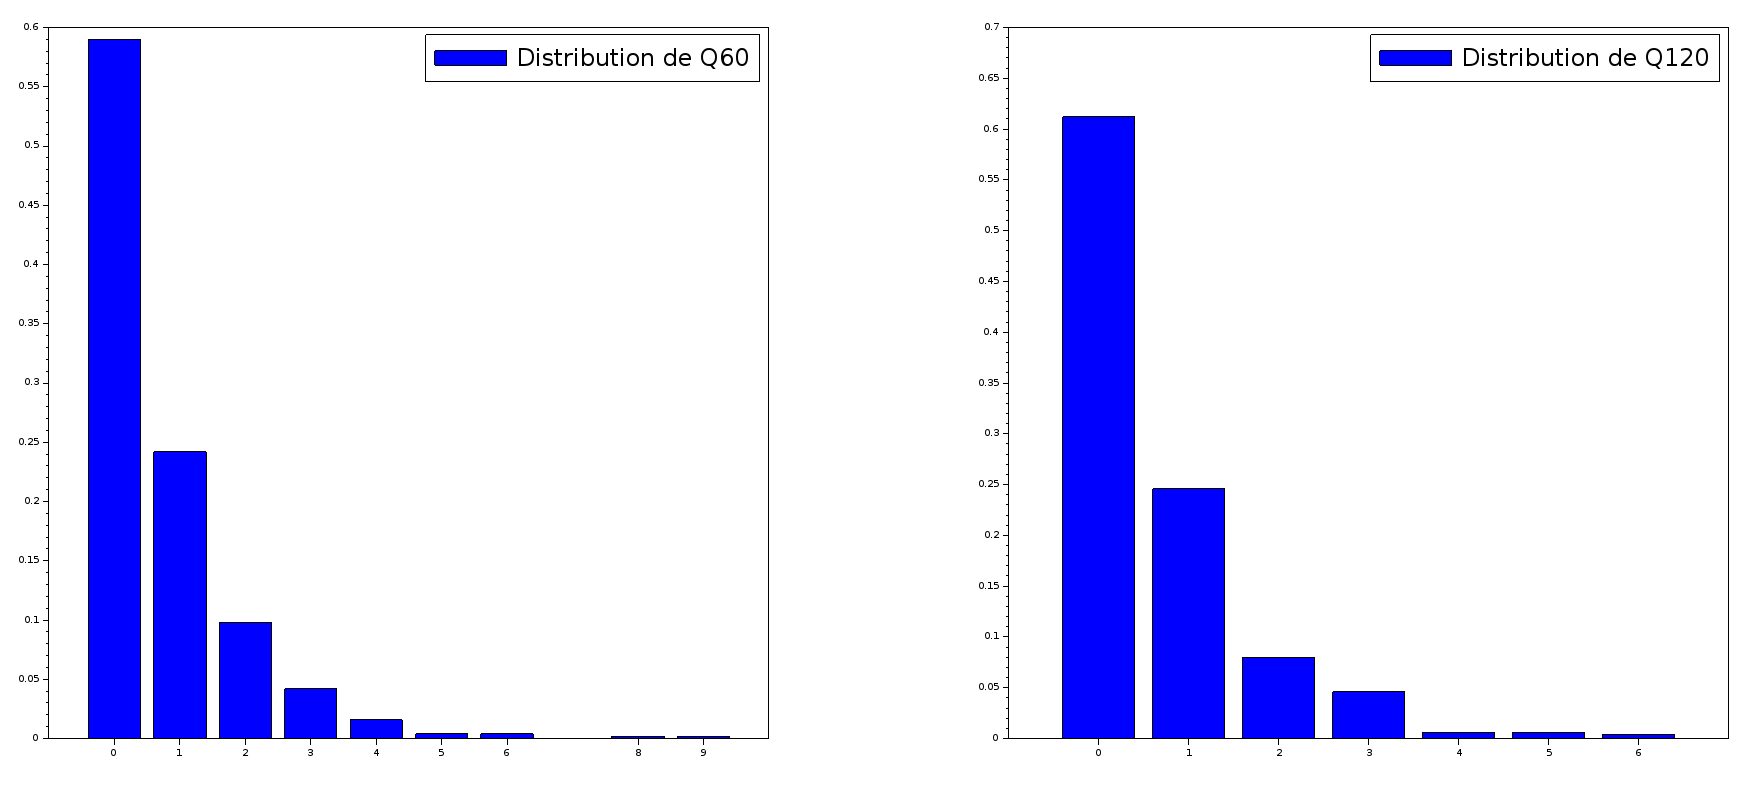
\includegraphics[width=425px]{img/inf/dist.png}
\end{center}
\begin{center}
	\begin{tabular}{c|cc}
		\hline \hline
		& Q60 & Q120 \\
		\hline
		mean() & 0.582 & 0.704 \\
		variance() & 0.9611984 & 1.1787415 \\
		\hline \hline
	\end{tabular}
\end{center}
\paragraph{} On peut bien voir d'après ces graphiques, que la file d'attente est toujours inférieure à 10 et majoritairement proche de 0, on en déduit que le serveur est donc sous-utilisé.

\subsubsection{Temps de service égaux en moyenne aux temps inter-arrivées}
\paragraph{Paramètre : $n=60$ ; $lambda=0.5$ ; $mu=0.5$}
\begin{center}
	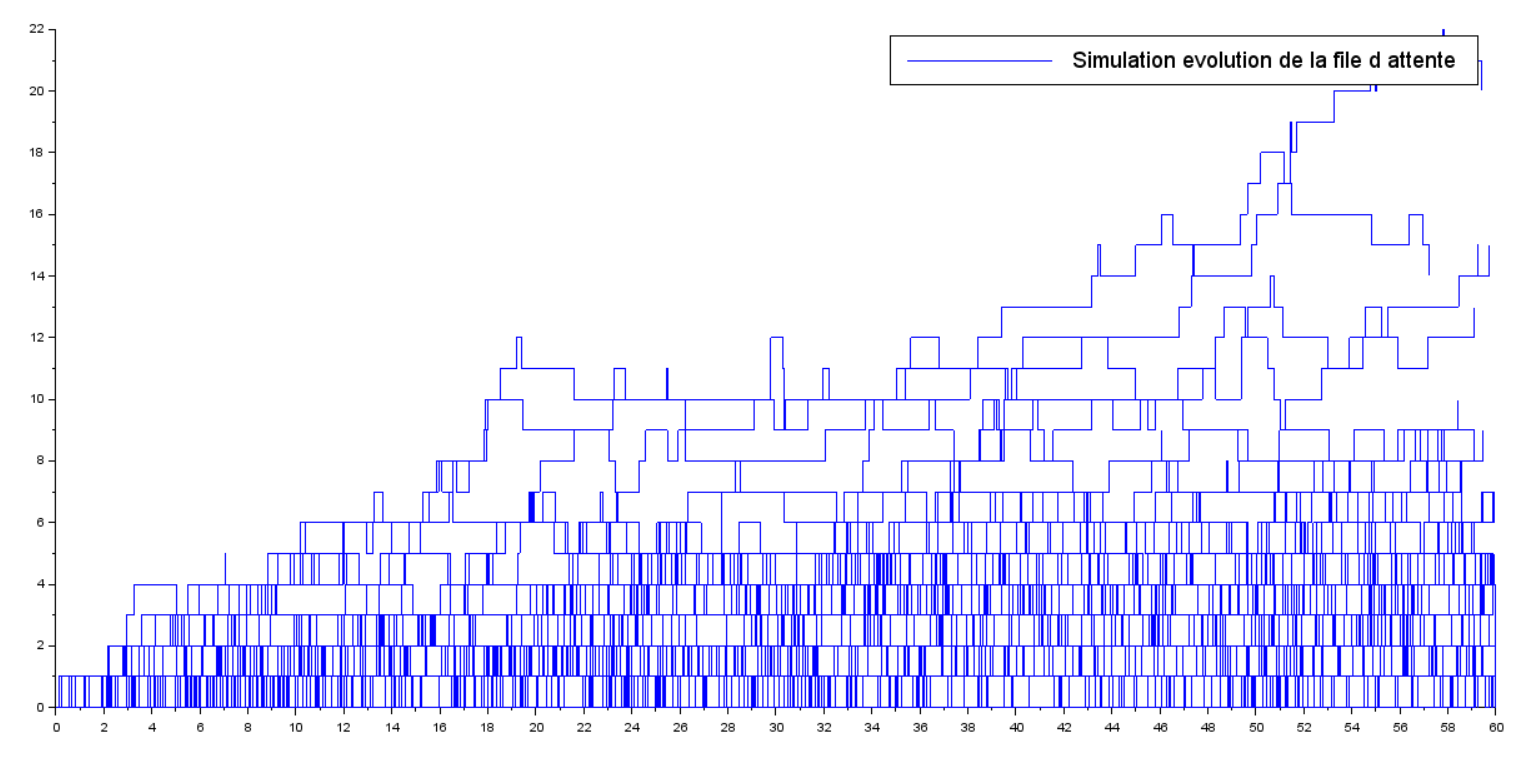
\includegraphics[width=425px]{img/egal.PNG}
\end{center}
\begin{center}
	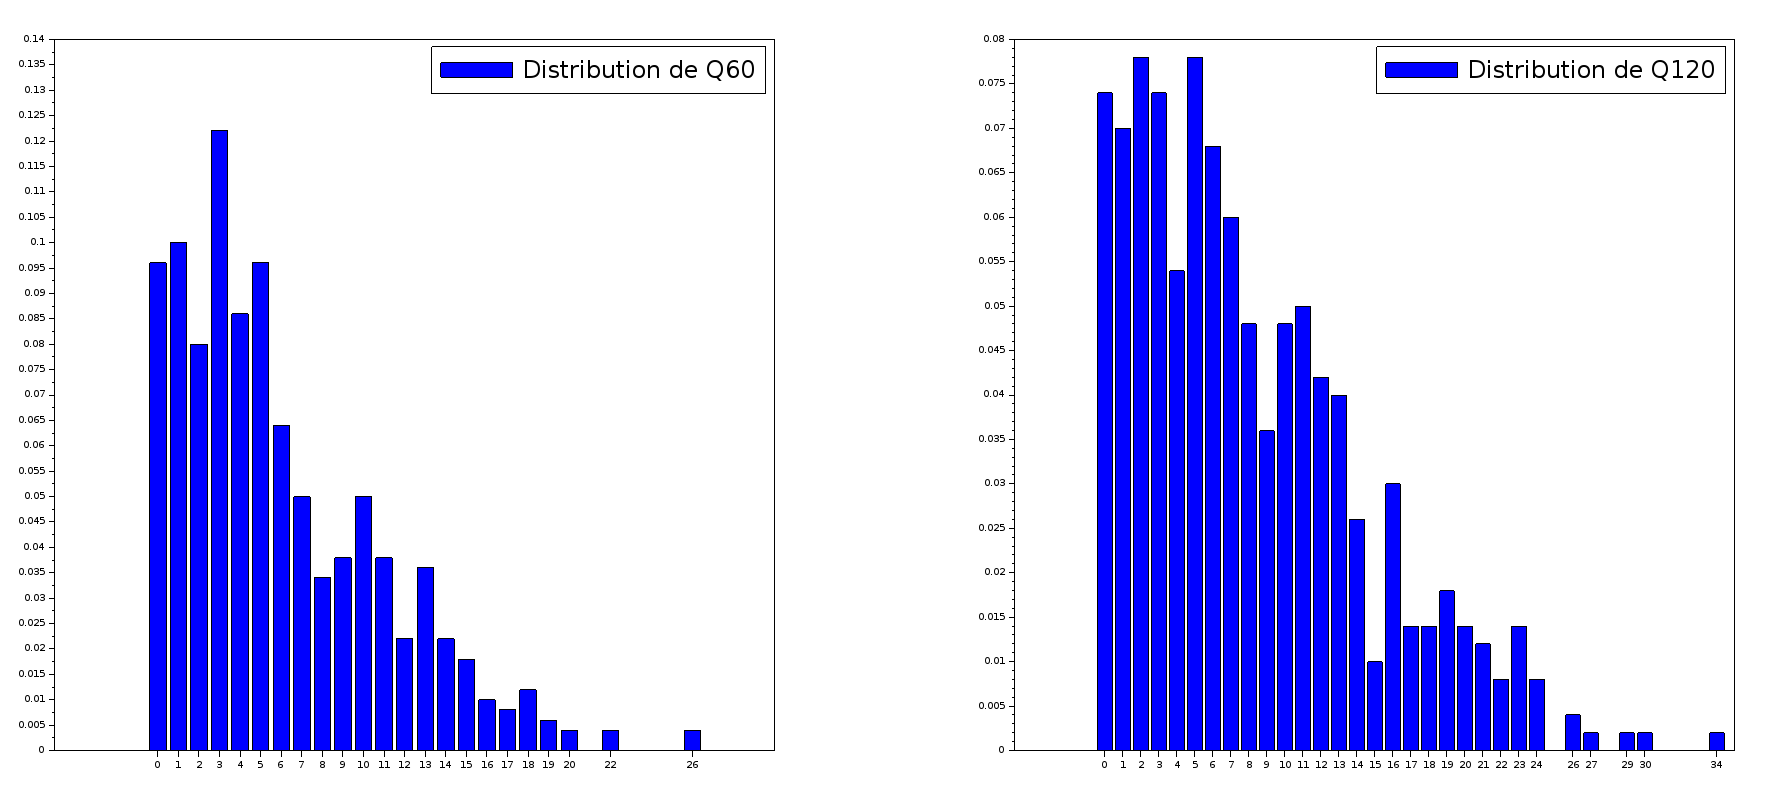
\includegraphics[width=425px]{img/egal/dist.png}
\end{center}
\begin{center}
	\begin{tabular}{c|cc}
		\hline \hline
		& Q60 & Q120 \\
		\hline 
		mean() & 5.726 & 8.476 \\
		variance() & 24.792509 & 46.350124 \\
		\hline \hline
	\end{tabular}
\end{center}
\paragraph{} On voit sur ces graphiques que la plupart des valeurs de la file d'attente sont entre 0 et 10, la taille de la file d'attente tend vers un régime stationnaire.

\section{Etude de la file à 3 serveurs}

\subsection{Simulation de stratégie circulaire}
\paragraph{}
Pour simuler la stratégie circulaire, on va utiliser la fonction $circul(Tmax,lambda,mu)$ où :
\begin{itemize}
	\item \textbf{Tmax} : Durée en seconde de la simulation
	\item \textbf{lambda} : $\lambda$ correspondant aux temps inter-arrivées
	\item \textbf{mu} : vecteur contenant les $\lambda$ correspondant aux temps de service des 3 serveurs
\end{itemize}
\begin{verbatim}
function [Q1, Q2, Q3] = circul(Tmax, lambda, mu)
    Q1 = [0, 0, 0]; Q2 = Q1; Q3 = Q1;
    i = 0; 
    ta = 0; 
    while (ta < Tmax)
        ia = randExp(1, lambda) 
        i = i+1 
        ta = ta + ia
        nq = modulo(i, 3) + 1
        ts = randExp(1, mu(nq))
        select nq 
        case 1.
            Q1 = insere(Q1, ta, ts)
        case 2 
            Q2 = insere(Q2, ta, ts)
        else
            Q3 = insere(Q3, ta, ts)
        end
    end
    Q1 = Q1(Q1(:,1)<Tmax,:)
    Q2 = Q2(Q2(:,1)<Tmax,:) 
    Q3 = Q3(Q3(:,1)<Tmax,:) 
endfunction 
\end{verbatim}
%
%\paragraph{}
%Dans cette fonction, on utilise 2 autres fonctions : 
%
%\begin{itemize}
%	\item $insere(q, ta, ts)$ où :
%	\begin{itemize}
%		\item \textbf{q} : File d'attente
%		\item \textbf{ta} : Instant d'arrivée de la requête
%		\item \textbf{ts} : Temps de service
%	\end{itemize}
%	\item $randExp(n, lambda) $
%	\begin{itemize}
%		\item \textbf{n} : taille du vecteur en sortie
%		\item \textbf{lambda} : $\lambda$ avec lequel sera générée la valeur aléatoire qui suit une loi exponentielle
%	\end{itemize}
%\end{itemize}

\begin{center}
	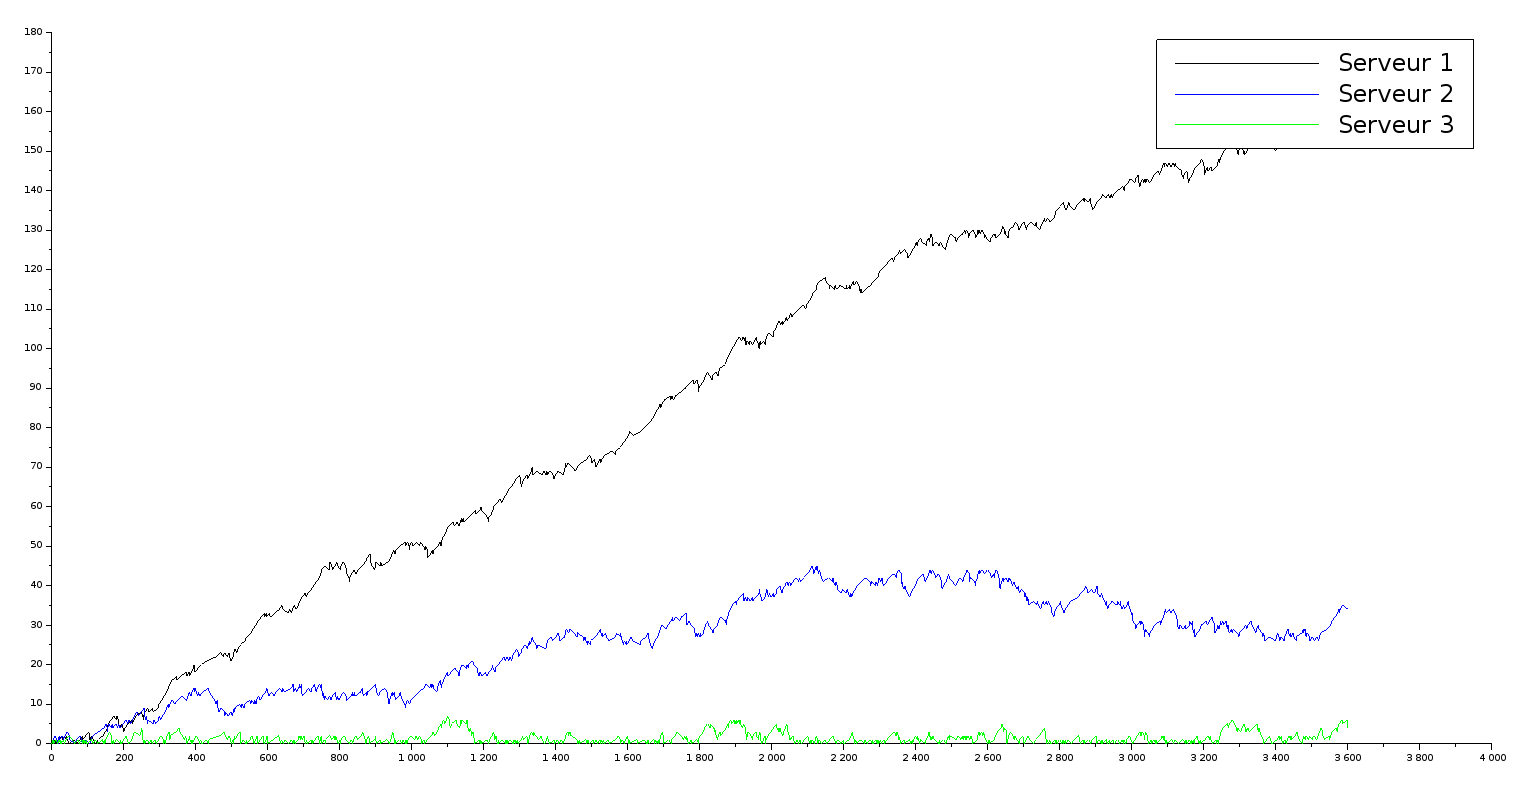
\includegraphics[width=425px]{img/circul1h.png}
\end{center}
\paragraph{Simulation sur 1 heure}

\begin{center}
	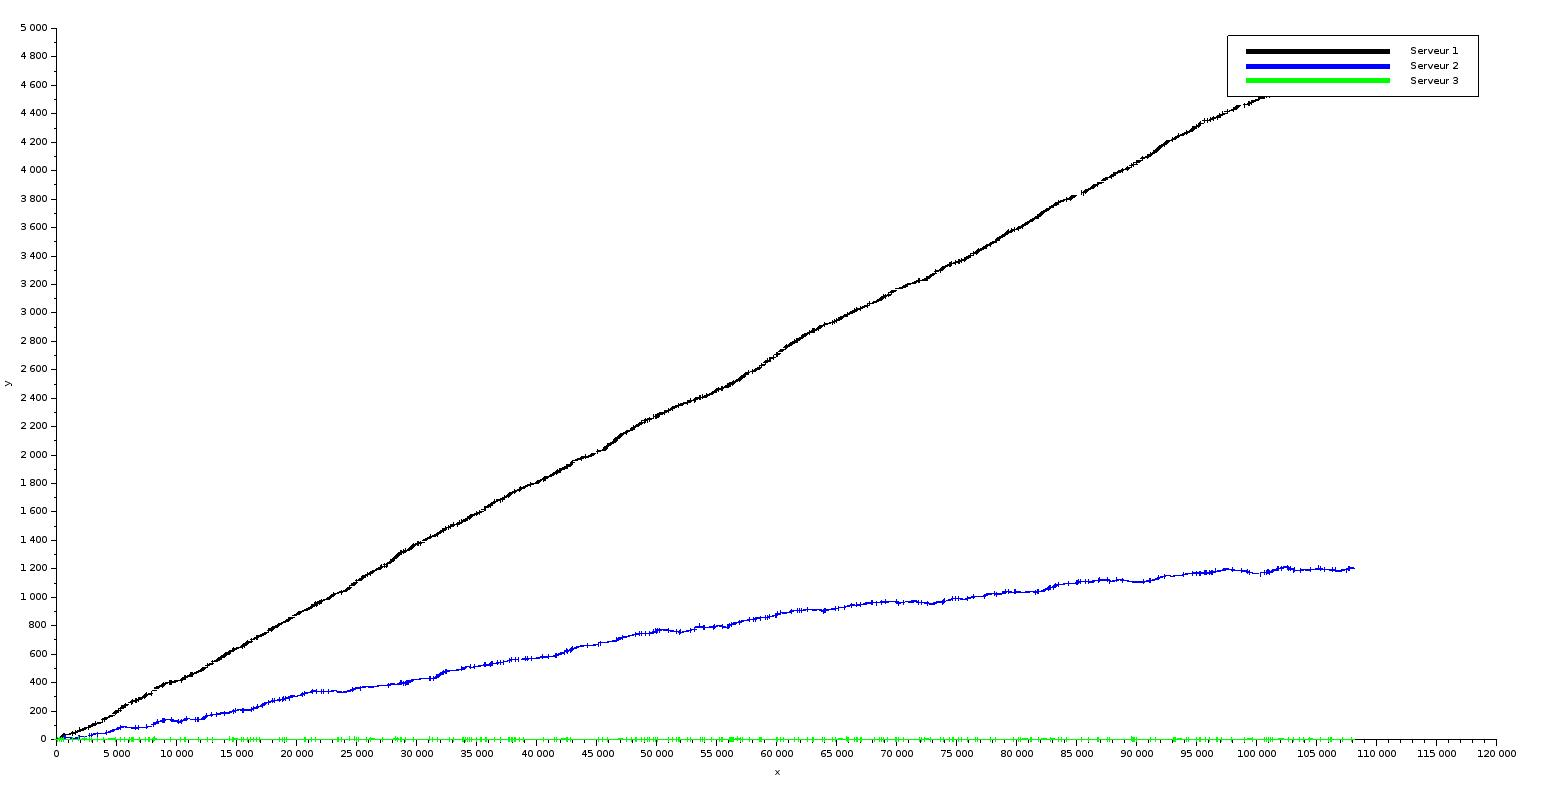
\includegraphics[width=425px]{img/circul30h.jpg}
\end{center}
\paragraph{Simulation sur 30 heures}
A partir de ces 2 graphiques, on peut clairement voir que :
\begin{itemize}
	\item Le serveur 3 est sous utilisé
	\item Le serveur 2 recoit légèrement trop de requete qu'il ne peut traiter, il finit par grimper doucement mais surement vers l'infini
	\item Le serveur 1 est complétement 'largué', la taille de sa fille d'attente croît de manière vertigineuse
\end{itemize}

\subsubsection{Etude numérique du temps de traversée du système pour une requête}

\paragraph{Outil de calcul}
Pour calculer les temps de traversée du système, on a créé une fonction Scilab $texecute(Q1,Q2,Q3)$ où :
\begin{itemize}
	\item \textbf{Q1,Q2,Q3} : correspondent aux représentation des files 
\end{itemize}
\begin{verbatim}
function [t1,t2,t3,t_mr] = texecute(Q1,Q2,Q3)
    //requetes sorties
    Q_s1 = Q1(Q1(:,3) == -1,1)
    Q_s2 = Q2(Q2(:,3) == -1,1)
    Q_s3 = Q3(Q3(:,3) == -1,1)

    //length file d'attentes requetes sorties
    l_s1 = length(Q_s1)
    l_s2 = length(Q_s2)
    l_s3 = length(Q_s3)

    //requetes entrées
    Q_re1 = Q1(Q1(:,3) == 1,1)
    Q_re2 = Q2(Q2(:,3) == 1,1)
    Q_re3 = Q3(Q3(:,3) == 1,1)

    //nb requetes entrées = nb requetes sorties
    Q_e1 = Q_re1(1:l_s1,1)
    Q_e2 = Q_re2(1:l_s2,1)
    Q_e3 = Q_re3(1:l_s3,1)

    //temps sortie - temps entrée 
    t_e1 = Q_s1 - Q_e1
    t_e2 = Q_s2 - Q_e2
    t_e3 = Q_s3 - Q_e3

    //temps moyen requete par serveur
    t1 = mean(t_e1)
    t2 = mean(t_e2)
    t3 = mean(t_e3)

    //temps moyen systeme
    t_mr = (t1+t2+t3)/3
endfunction
\end{verbatim}

\paragraph{Résultats pour une simulation}
Les résultats peuvent varier, mais sont proches de ces résultats :
\begin{center}
	\begin{tabular}{c|ccc|c}
		\hline \hline
		& Serveur 1 & Serveur 2 & Serveur 3 & Tous \\
		\hline
		moyenne & 820.60768 & 246.56614 & 12.08801 & 359.75394 \\
		\hline \hline
	\end{tabular}
\end{center}

\subsubsection{Etude numérique du nombre de requêtes dans le système}

\begin{center}
	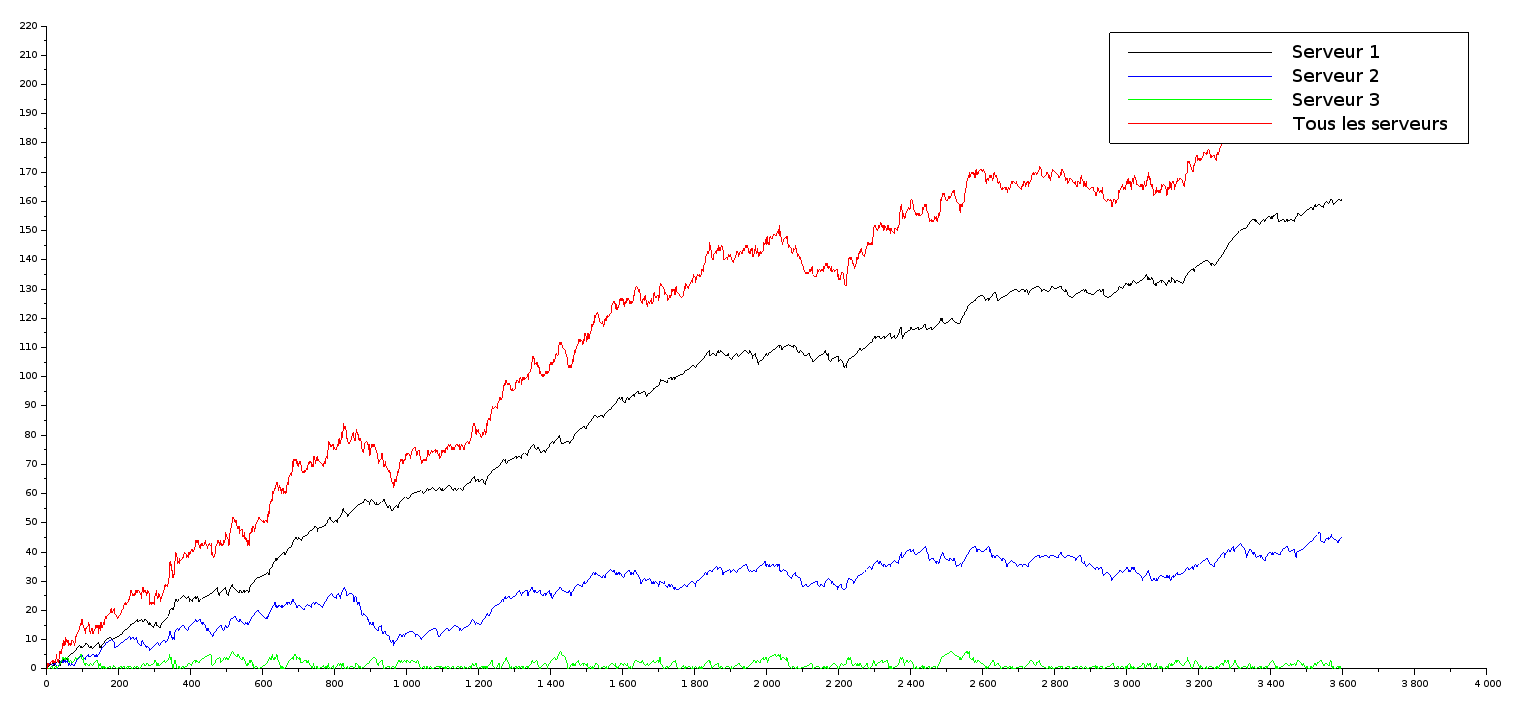
\includegraphics[width=425px]{img/tls.png}
\end{center}
\hyperref[tls]{Lien vers le code}

\subsubsection{Recherche d'un régime stationnaire}

\paragraph{}
Au vu des résultats, on peut en conclure que la stratégie circulaire n'est pas du tout optimale, on remarque aisément que la taille de la file d'attente du service ne fait que croite sans jamais se stabiliser.
\paragraph{}
On va donc chercher d'autres stratégies qui seraient plus adaptés et plus optimale pour le service.

\subsection{Simulation de la stratégie d'affection aléatoire proportionnelle}
\subsubsection{Simulation}

\paragraph{}
Pour simuler la stratégie d'affectation aléatoire proportionnelle, on utilise la fonction $aleaProp(Tmax,lambda,mu)$ où :
\begin{itemize}
	\item \textbf{Tmax} : Durée en seconde de la simulation
	\item \textbf{lambda} : $\lambda$ correspondant aux temps inter-arrivées
	\item \textbf{mu} : vecteur contenant les $\lambda$ correspondant aux temps de service des 3 serveurs
\end{itemize}
\begin{verbatim}
function [Q1, Q2, Q3] = aleaProp(Tmax, lambda, mu)
    Q1 = [0, 0, 0]; Q2 = Q1; Q3 = Q1;
    i = 0;
    ta = 0;
    while (ta < Tmax)
        ia = randExp(1, lambda)
        i = i+1
        ta = ta + ia 
        nq = num_serv() 
        ts = randExp(1, mu(nq))
        select nq
        case 1
            Q1 = insere(Q1, ta, ts)
        case 2 
            Q2 = insere(Q2, ta, ts)
        else
            Q3 = insere(Q3, ta, ts)
        end
    end
    Q1 = Q1(Q1(:,1)<Tmax,:)
    Q2 = Q2(Q2(:,1)<Tmax,:) 
    Q3 = Q3(Q3(:,1)<Tmax,:) 
endfunction 
\end{verbatim}

\paragraph{}
Dans la fonction précédente, on utilise la fonction suivante : $num\_serv()$, qui génére le numéro de serveur à allouer généré aléatoirement de manière proportionnelle aux temps de service des différents serveurs.

\begin{verbatim}
function nq = num_serv()
    u = rand()
    if u < 0.2 then
        nq = 1
    elseif u < 0.5
        nq = 2
    else
        nq = 3
    end
endfunction
\end{verbatim}

\paragraph{Résultats}
\begin{center}
	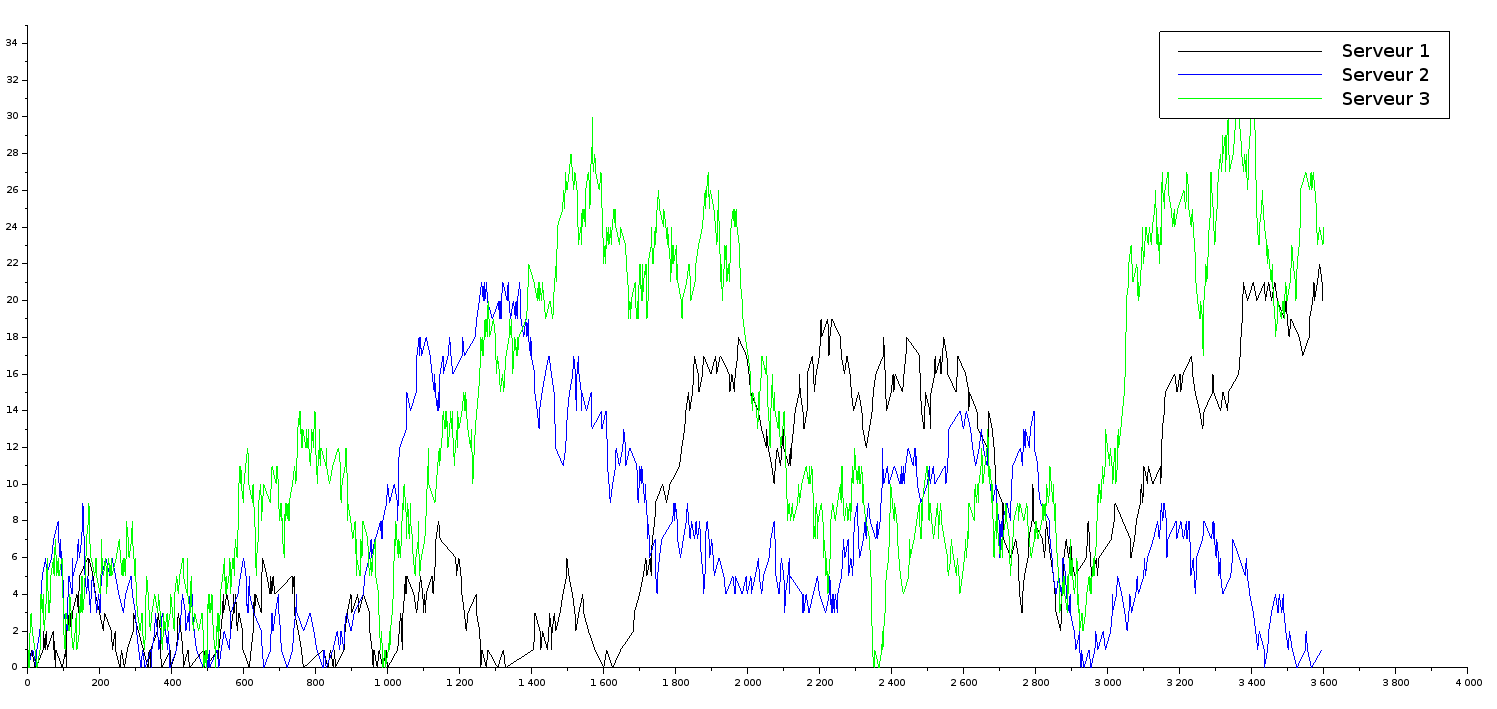
\includegraphics[width=425px]{img/aleaProp.png}
\end{center}

\paragraph{Représentation de l'évolution des files d'attente pendant 20 heures}
\begin{center}
	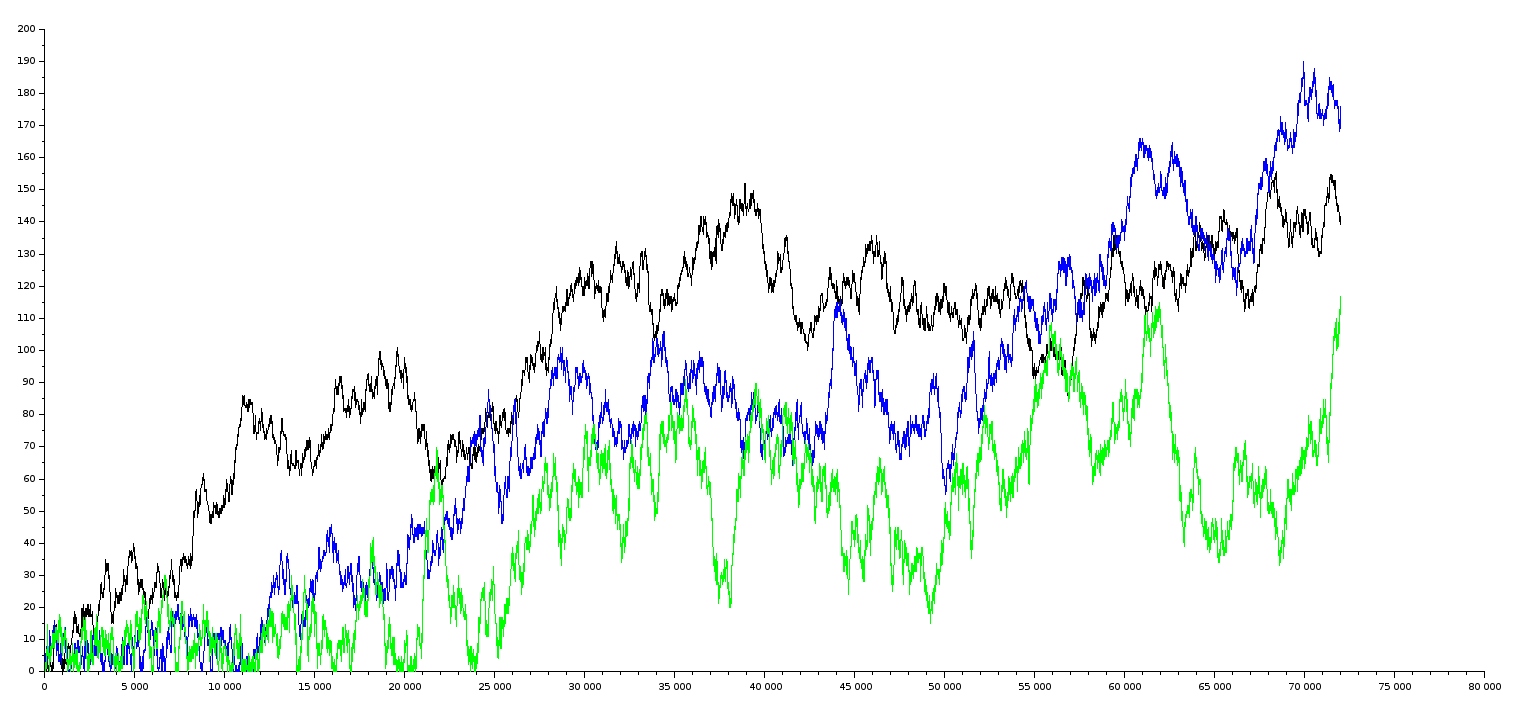
\includegraphics[width=425px]{img/alea20h.png}
\end{center}

\subsubsection{Etude numérique du temps de traversée du système pour une requête}

\paragraph{Résultats pour une simulation}
Les résultats peuvent varier, mais sont proches de ces résultats :
\begin{center}
	\begin{tabular}{c|ccc|c}
		\hline \hline
		& Serveur 1 & Serveur 2 & Serveur 3 & Tous \\
		\hline
		moyenne & 182.58103 & 101.34571 & 115.17009 & 133.03228 \\
		\hline \hline
	\end{tabular}
\end{center}
\paragraph{}
On remarque que les résultats semblent plus équilibrés, et que les serveurs sont généralement mieux utilisés qu'avec la stratégie circulaire.

\subsubsection{Etude numérique du nombre de requêtes dans le système}

\subsection{Autres stratégies, aléatoires ou/et déterministes}

\subsubsection{Stratégie semi-circulaire}
%\begin{center}
%	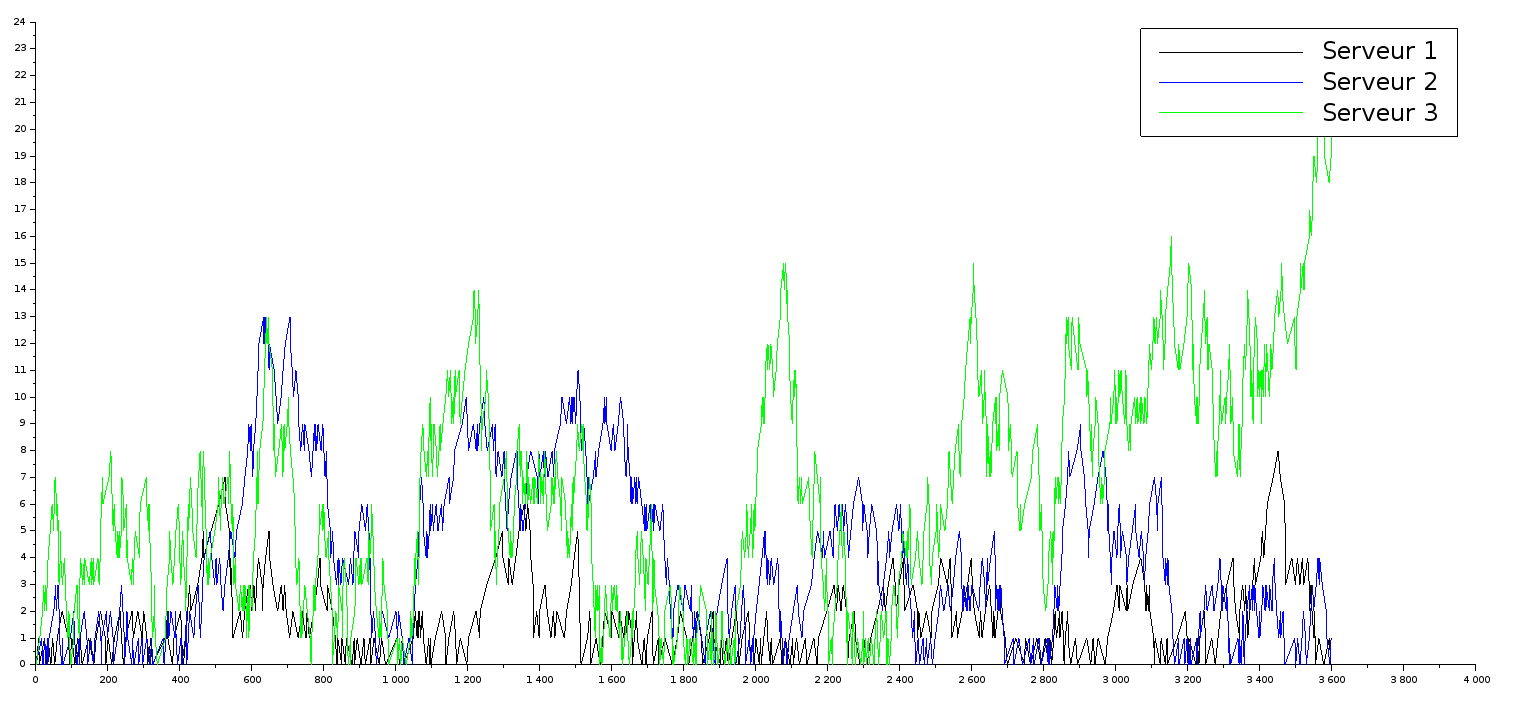
\includegraphics[width=425px]{img/semiCirculaire.png}
%\end{center}

\begin{tabular}{c|ccc}
	\hline \hline
	Choix du serveur & Temps restants S1 & Temps restants S3 & Temps restant S2 \\
	\hline 
	1 & 15 \\
	3 & 12 & 6 \\
	2 & 9 & 3 & 10 \\
	3 & 6 & 6 & 7 \\
	3 & 3 & 9 & 4 \\
	1 & 15 & 6 & 1 \\
	2 & 12 & 3 & 10 \\
	3 & 9 & 6 & 7 \\
	3 & 6 & 9 & 4 \\
	2 & 3 & 6 & 11 \\
	\hline
	\textbf{1} & \textbf{15} & \textbf{3} & \textbf{8} \\
	3 & 12 & 6 & 5 \\
	2 & 9 & 3 & 12 \\
	3 & 6 & 6 & 9 \\
	3 & 3 & 3 & 6 \\
	1 & 15 & 0 & 3 \\
	2 & 12 & 0 & 10 \\
	3 & 9 & 6 & 7 \\
	3 & 6 & 9 & 4 \\
	2 & 3 & 6 & 11 \\
	\hline
	\textbf{1} & \textbf{15} & \textbf{3} & \textbf{8} \\
	3 & 12 & 6 & 5 \\
	... & ... & ... & ... \\
	\hline \hline
\end{tabular}

\paragraph{}
La solution que nous proposons ici est une solution déterministe, semi-circulaire, basée sur une suite d'attribution optimisée.
Pour ce faire, nous sommes partis d'une idée simple: attribuer les requêtes aux différents serveurs, en choisissant à chaque fois le serveur qui présente le temps de traitement restant le plus petit.
\paragraph{}
Ainsi, au fur et à mesure des attributions, il en ressort une suite récurrente composée de 10 éléments :
\begin{center}
	$[1,3,2,3,3,1,2,3,3,2]$
\end{center}
\paragraph{}
On parcourt ensuite cette suite pour obtenir un ordre d'attribution plutôt optimisé.

\paragraph{}On obtient donc la fonction suivante $semicircul(Tmax,lambda,mu)$:
\begin{verbatim}
function [Q1, Q2, Q3] = semicircul(Tmax, lambda, mu)
    Q1 = [0, 0, 0]; Q2 = Q1; Q3 = Q1;
    tab=[1,3,2,3,3,1,2,3,3,2];  
    ta = 0;
    while (ta < Tmax)
        for i=1:10
            nq=tab(i);
            ia = randExp(1, lambda) 
            ta = ta + ia 
            ts = randExp(1, mu(nq)) 
            select nq 
            case 1 
                Q1 = insere(Q1, ta, ts)
            case 2
                Q2 = insere(Q2, ta, ts)
            else
                Q3 = insere(Q3, ta, ts)
            end
        end
    end
    Q1 = Q1(Q1(:,1)<Tmax,:)
    Q2 = Q2(Q2(:,1)<Tmax,:) 
    Q3 = Q3(Q3(:,1)<Tmax,:) 
endfunction 
\end{verbatim}

\paragraph{Résultat de la simulation}
\begin{center}
	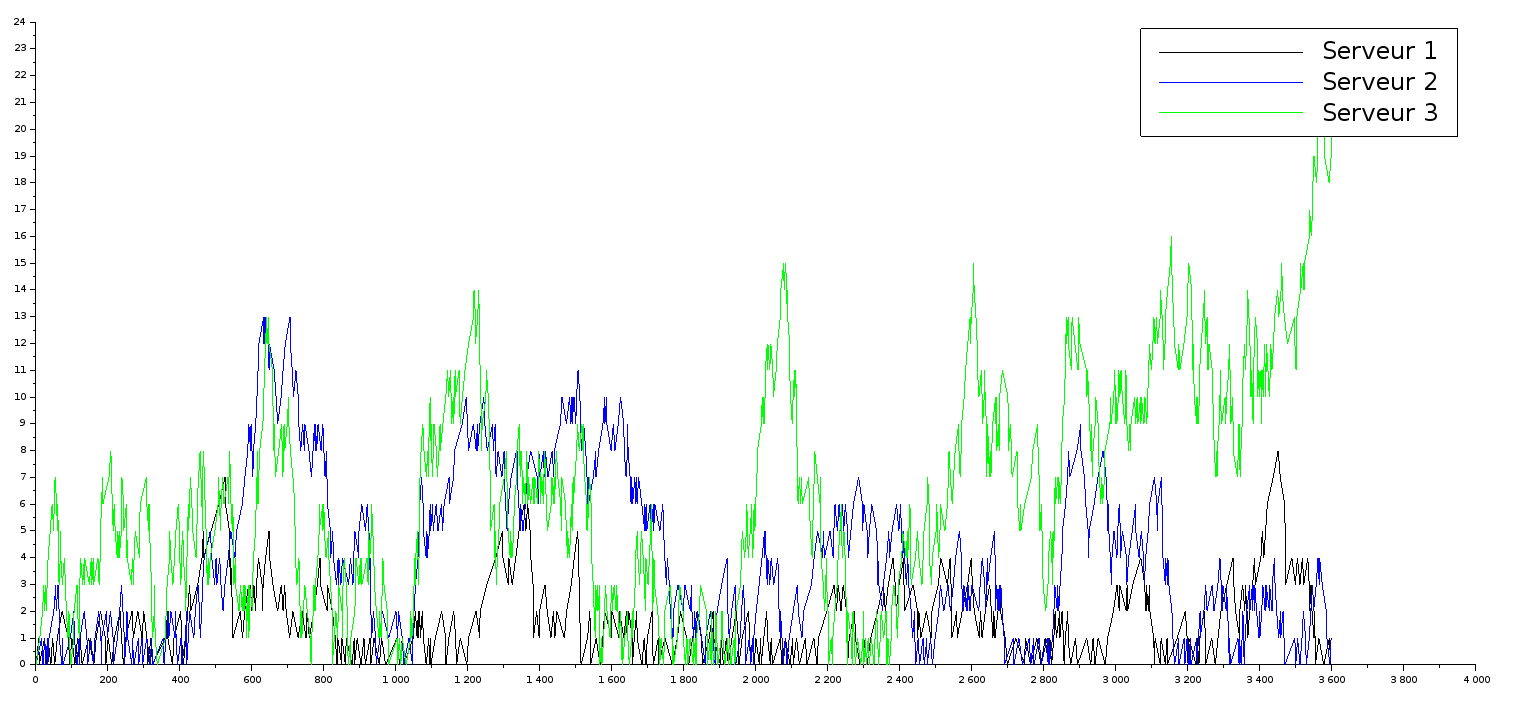
\includegraphics[width=425px]{img/semiCirculaire.png}
\end{center}

\subsubsection{Stratégie d'attribution selon la taille de la file d'attente}

\paragraph{}
Cette solution pour l'attribution des requêtes aux différents serveurs fonctionne de la sorte :  pour chaque nouvelle requête, on observe le nombre de requêtes file d'attente de chaque serveur. On pondère ensuite ce nombre par le temps de traitement des requêtes moyen de chaque serveur. On choisit finalement le serveur qui obtient le plus petit résultat pour lui attribuer la nouvelle requête.

\paragraph{}On obtient donc la fonction suivante $choix(Tmax,lambda,mu)$:
\begin{verbatim}
function [Q1, Q2, Q3] = choix(Tmax, lambda, mu)
    Q1 = [0, 0, 0]; Q2 = Q1; Q3 = Q1;
    i = 0;
    ta = 0; 
    while (ta < Tmax)
        ia = randExp(1, lambda)
        i = i+1 
        ta = ta + ia 
        ind1 = sum(Q1(:,1)<ta)// on récupère les files d'attentes de chaque serveur
        ind2 = sum(Q2(:,1)<ta)
        ind3 = sum(Q3(:,1)<ta)
        tq1 = Q1(ind1,2)
        tq2 = Q2(ind2,2)
        tq3 = Q3(ind3,2)
        minserv=min(tq1,tq2,tq3)
        if tq1 == minserv then // enfin on choisit le serveur qui a le plus petit résultat
            nq = 1
        elseif tq2 == minserv
            nq = 2
        else
            nq = 3
        end
        ts = randExp(1, mu(nq))
        select nq 
        case 1 
            Q1 = insere(Q1, ta, ts)
        case 2 
            Q2 = insere(Q2, ta, ts)
        else
            Q3 = insere(Q3, ta, ts)
        end
    end
    Q1 = Q1(Q1(:,1)<Tmax,:)
    Q2 = Q2(Q2(:,1)<Tmax,:)
    Q3 = Q3(Q3(:,1)<Tmax,:)
endfunction
\end{verbatim}

\paragraph{Résultat de la simulation}
\begin{center}
	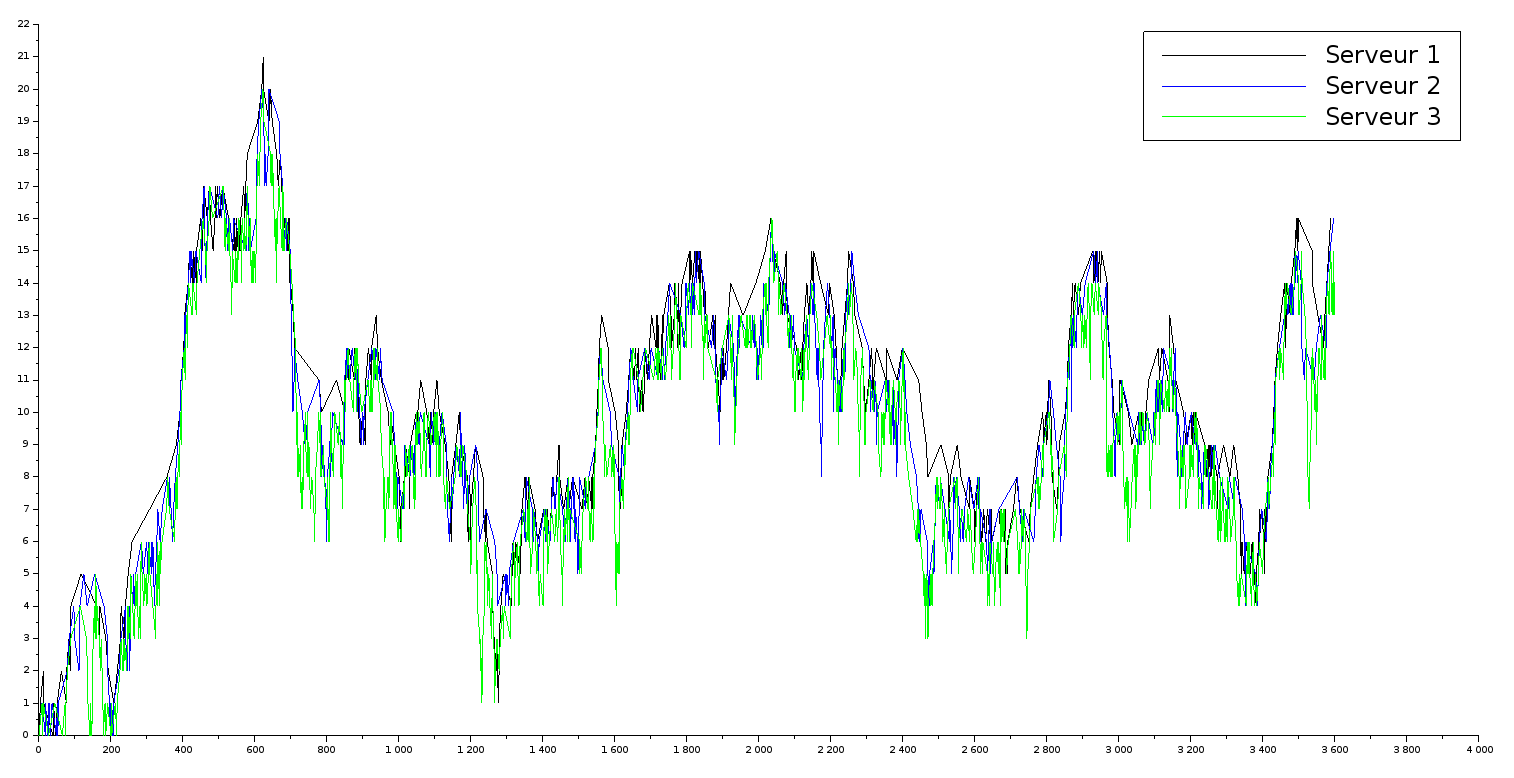
\includegraphics[width=425px]{img/choix.png}
\end{center}

\section{Conclusion}
\paragraph{}

\newpage
\appendix

\section{Stratégie circulaire - Etude numérique du nombre de requêtes dans le système}\label{tls}
%
%\subsection{}
\begin{verbatim}
plot2d(Q1(:,1), Q1(:,2), style= 1)
plot2d(Q2(:,1), Q2(:,2), style= 2)
plot2d(Q3(:,1), Q3(:,2), style= 3)

Q=[Q1;Q2;Q3]
Qt=[0,0,0]
Qt=gsort(Q,'r','i')
total=0;
for i=1:length(Q(:,1))
Qt(i,2)=total;
[a,b]=find(Q(:,1)==Qt(i,1),1);
increment=Q(a,3);
Qt(i,3)=increment;
total=total+increment
end

plot2d(Qt(:,1), Qt(:,2), style = 5)

legend("Serveur 1","Serveur 2","Serveur 3", "Tous les serveurs")
\end{verbatim}
%
\end{document}